\section{Changing all parameters}\label{sec:change}
reduced graph, 15700 samples

\begin{figure}[hbt!]\centering
    \subfloat[]{\label{}
    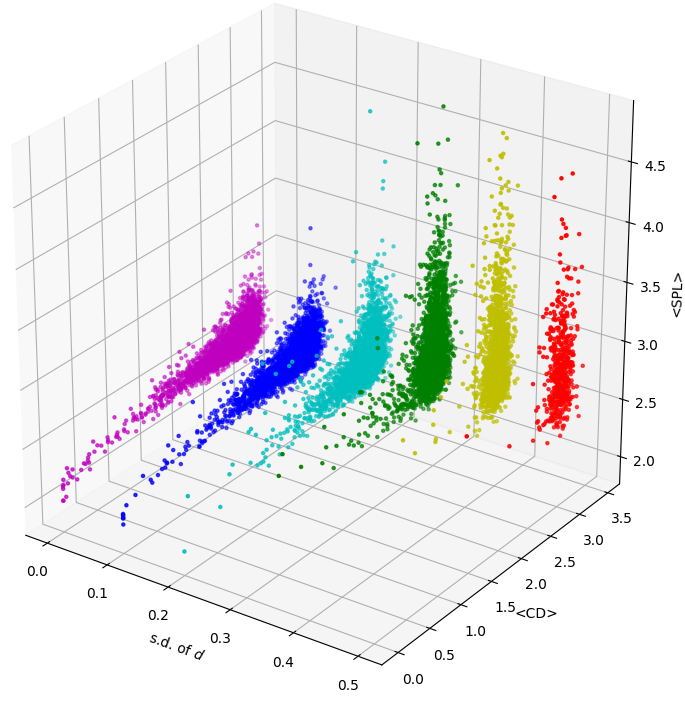
\includegraphics[width=.45\linewidth]{images/change_all stdd.png}}
    \caption{3D scatter plot showing the effect on SPL and CD of each
    standard deviation of
    (a) $d$. Each dot is the result of one simulation run, colored
    according to the standard deviation value.}
    \label{figure}
\end{figure}


\subsection{Regression and Comparison with Base}

\begin{gather}\label{eq:cared}
    <CD> ~ \thicksim ~ 2.27 + 1.75\sd + 1.32\sr - 0.18\sw -
                2.97\ds - 0.20\dw - 0.27\ssw \label{ca1}\\
    <SPL_s> ~ \thicksim ~ 2.34 + 1.05\sd + 0.13\sr + 0.11 \sw +
                0.28\ds - 0.004\dw + 0.14\ssw \label{ca2}
\end{gather}

